\documentclass[conference]{IEEEtran}
\usepackage{xcolor}
\usepackage[english]{babel}
\usepackage[utf8]{inputenc}
\usepackage[style=numeric]{biblatex}
\addbibresource{../literature.bib}% Syntax for version >= 1.2
\usepackage{graphicx}
\graphicspath{{../images/}}

\newcommand{\fixnote}[2]{\textbf{\color{red}{FIX}}\footnote{{\bf #1:} #2}}
\newcommand{\fix}[2]{{\color{red} {\bf tofix:} #2}}
% \renewcommand{\fixnote}[2]{}
% \renewcommand{\fix}[2]{}

\begin{document}
\title{On Etiology of Cybersecurity}

\author{\IEEEauthorblockN{Marco Rocchetto}
\IEEEauthorblockA{V-Research\\
Verona, Italy\\
Email: marco@v-research.it}
\and
\IEEEauthorblockN{Francesco Beltramini}
\IEEEauthorblockA{V-Research\\
Verona, Italy\\
Email: francesco@v-research.it}
}

\maketitle

\begin{abstract}
The abstract goes here.
\end{abstract}

\IEEEpeerreviewmaketitle

\section{Introduction}\label{sec:intro}
In \cite{Herley2016unfalsifiability}, Cormac Herley explores what he calls
``an asymmetry in computer security'', which he defines as follows: ``Things
can be declared insecure by observation, but not the reverse. There is no
observation that allows us to declare an arbitrary system or technique
secure''. Herley then uses this argument to show that ``claims that any measure
is necessary for security are empirically unfalsifiable''. Given that, any
theory which is not falsifiable by an empirical experiment is well
known\footnote{``A theory which is not refutable by any conceivable event is
nonscientific. Irrefutability is not a virtue of a theory (as people often
think) but a vice.'' -- Karl Popper, Conjectures and
Refutations \cite{popper1962conjectures}} to be nonscientific (i.e.
unfalsifiability is a fallacy of a theory), Herley concludes that there is no
scientific theory on cybersecurity; which means that cybersecurity lays in the
realm of pseudo-sciences \cite{Herley2016usenixvideo}.  Herley, e.g.
in \cite{Herley2017justifying}, discusses the implications of a
nonscientific approach to cybersecurity, and highlights the tremendous impact on
all the scientific research and engineering of systems; leading often to
terrorism and wars, and wasting of resources in useless protections or
overspending.  While the criticism is investigated
in \cite{Herley2016unfalsifiability}, no solution is provided nor envisioned.  On the
contrary, the goal of this work is to lay the foundations of a
scientific cybersecurity theory. 

We consider the problem raised by Herley not confined to
``computer security'' but to any abstract system (so that our theory may hold
for any sound implementation such as networks, mechanical, cyber, or
cyber-physical system, or even a single computer or a single device such as an
hard-drive).  There is also an apparent inconsistency in
\cite{Herley2016unfalsifiability} that we seek to clarify before following (as
we agree) the scientific path draw by Herley: cybersecurity is defined as an
abstract property in many formal approaches to the investigation of the
security of systems, and the security of the design of a formally verified
protocol is indeed falsifiable (against the security properties verified).  For
example, in the protocol verification community, security is often defined as a
formalization of the high-level properties confidentiality, integrity, and
availability. The problem in such approaches is not the definition of what
cybersecurity is but the generality of the results, since they tackle a specific
step (and not the first) of the engineering process (of systems).  Therefore,
the theories underlying the verification are based on assumptions which
non-evidently apply to a general security theory.  As an example, the so called
Dolev-Yao attacker model\footnote{For the sake of simplicity, the Dolev-Yao
attacker can be considered as an abstraction of an active attacker who controls
the network but cannot break cryptography.} \cite{Dolev1983security} only
applies to specific instances (often called scenarios) and abstraction of the
protocol. This, in turn, creates a false sense of security since requires
non-justifiable assumptions on the abstraction of the system of which security
is verified. More specifically, for the formal security verification of a
system in which two or more agents are communicating, a formalized scenario
needs to be defined by a modeler who chooses (among others): (i) a scope of the
formalization (e.g.  excluding the server that distributes the public key is
often done when verifying the security of authentication protocols), (ii) the
number of sessions (even tough some approaches do reason on an infinite number
of sessions such as \cite{Escobar2007maudenpa}), (iii) honesty/dishonesty of
the peers (e.g.  in the ASLan++ language \cite{Oheimb2010aslan++}), and (iv)
the abstraction of the cryptographic primitives (e.g.  ProVerif vs CryptoVerif
\cite{Blanchet2017symbolic}).  While many tools and theories improves those 
issues, there is no agreement on which should be the definitive
approach (if any). More importantly, some of the choices made by the
modelers/engineers using those formal approaches may completely change the
results of the formal verification of the system (an interesting example on how
difficult it is to even just compare the approaches is given in
\cite{Cremers2009comparing}). 
\begin{figure}[t]
	\centering
	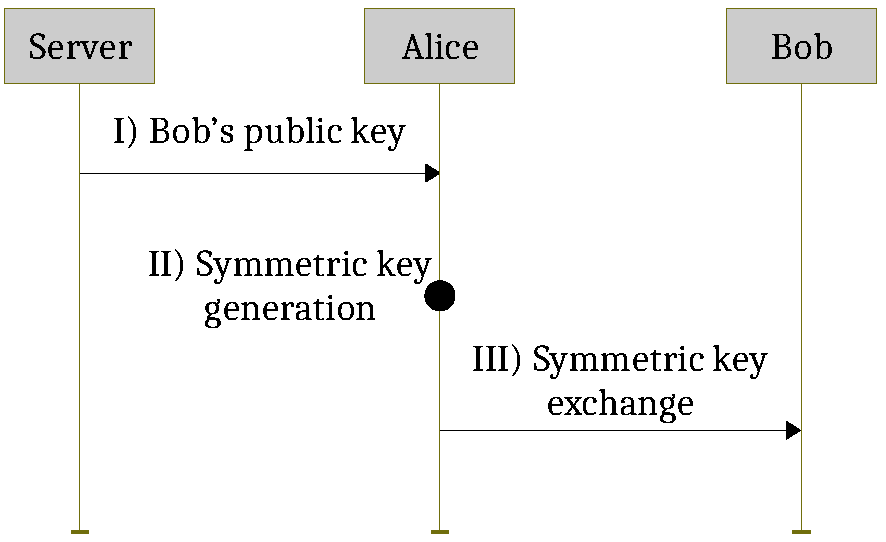
\includegraphics[width=.7\columnwidth]{protocol-example.pdf}
	\caption{Abstraction of an ad-hoc esemplificative protocol execution}
	\label{fig:protocol-example}
\end{figure}
For example, in Figure~\ref{fig:protocol-example}, under the perfect
cryptography assumption\footnote{As defined in \cite{Rocchetto2016cpdy}: ``In
the so called perfect cryptography assumption, the security encryption scheme
is suppose to be perfect, without any exploitable flaw, and so the only way for
the attacker to decrypt a message is by using the proper key. That assumption
is widely accepted in the security protocol community, and most of the formal
reasoning tools for the analysis of security protocols abstract away the
mathematical and implementation details of the encryption scheme
\cite{Turuani2006clatse,Basin2005ofmc,Armando2016satmc,Rocchetto2017interpolation}''}
and assuming that no violation to any security property is done after message
I), the freedom of choosing the scope
determines that the flaws related to the dishonest impersonation of the Server
may or may not be considered in the verification process.  This choice has
tremendous impact on the focus and findings of the verification of the security
of the protocol.  While this may seem to turn upon minutiae and foreseeable,
this highlights the false sense of security that may derive from a
non-falsifiable theory of system security\footnote{``To the superficial
observer, the analysis of these forms seems to turn upon minutiae. It does in
fact deal with minutiae, but they are of the same order as those dealt with in
microscopic anatomy.'' -- Karl Marx, Capital Volume 1, 1867}.

\paragraph{Structure} We start, in
Section~\ref{sec:literature}, by detailing the problem statement, reporting a
literature review on the main concepts and definitions related to security.  We
formulate a security hypothesis in Section~\ref{sec:hypothesis}; which we use
to propose a theory on system security in Section~\ref{sec:theory}. In
Section~\ref{sec:secra}, we apply our theory for the tool-assisted security
risk assessment of a CPS (with an ad-hoc example, based on the SWaT testbed
\cite{Mathur2016swat}).  This application shows how our theory can be used to
predict all of the possible security weaknesses of a system, allowing the
falsification of our theory.  In fact, if any security weaknesses were to be
found in a system and not predicted by our theory, the theory could be declared
incomplete.  Similarly, if a security weakness would be predicted by our theory
but found to be impossible to have our theory could be declared as wrong.

\section{Literature Review}\label{sec:literature}
\begin{figure*}[t]
	\centering
	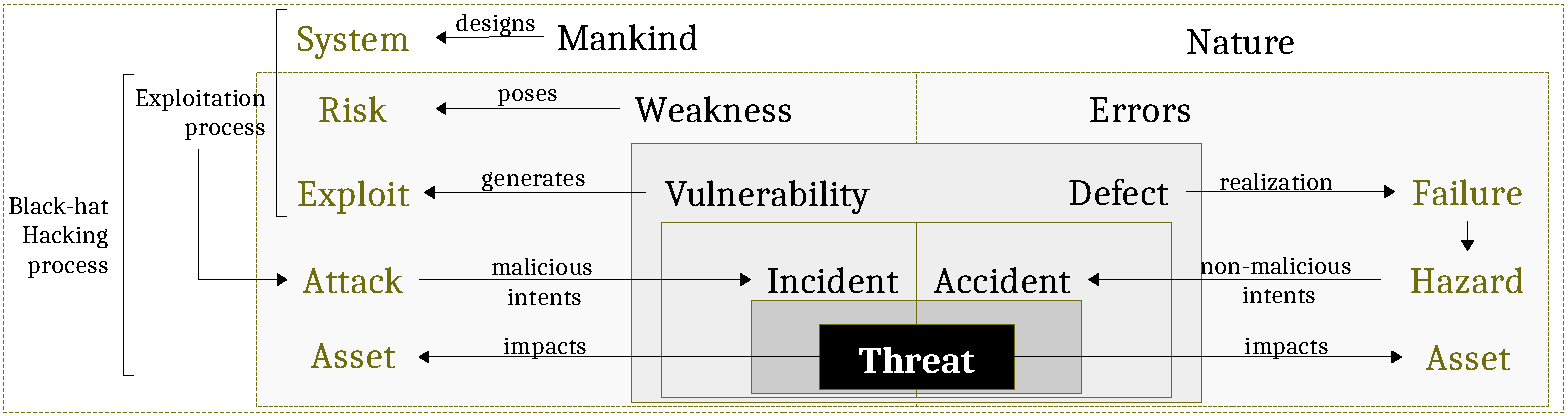
\includegraphics[width=\textwidth]{safety-security_3.pdf}
	\caption{Overview of keywords related to security and safety}
	\label{fig:safety-security}
\end{figure*}

\fixnote{mr}{add weakness-error in picture and text}
In most of the natural languages the concepts of safety
and security are not syntactically differentiated and both terms (safety and
security) are expressed by the same word, e.g. sicurezza in Italian.  A
semantic distinction between safety and security is correlated to a
belief\footnote{A belief has to be intended as a proposition which is supposed
to be true by the majority of people in our society, without a scientific
underlying theory but based on partial empirical evidences or inductive reasoning based on partial empirical evidences.} that
safety deals with \emph{accidents} (i.e. an unfortunate incident) posed by the
natural environment (e.g. natural events such as wearing of hardware
components) while security deals with \emph{incidents} posed by mankind (e.g.
attackers and bugs).  The fundamental difference between nature and mankind (and,
in turn, between safety and cybersecurity) is believed to be on the different
intents\footnote{``The belief–desire–intention software model (BDI) is a
software model developed for programming intelligent
agents.''\cite{wiki-bdi}. In the BDI model, the intents represents the
deliberative state of an agent which determines the choice of that agent on
what to do.} (accidents are unfortunate while incidents are not) of the causes
that generates a threat; namely, nature is believed not to have malicious
intents (but unfortunate causes-effects) while threats generated by mankind are
malicious\footnote{Of course, logical flaws or bugs may be
introduced by other means (e.g. ignorance) without explicit malicious intents,
but the exploitation of those flaws is considered (for now, and detailed
afterwards in the article) malicious, and then we consider any vulnerability to
be malicious even if due to the lack of skills.}.
This conclusion seems to be against a general formulation of a cybersecurity theory;
how can we define a theory that predicts what a human being will do?
The cybersecurity attacks seems to be related to the creativity of the attacker
and then unpredictable. Currently, our understanding of cybersecurity is
stored into a network of databases of weaknesses (e.g.
CWE\cite{MITRE2020CWEresearch}), vulnerabilities (e.g. CVE\cite{CVE},
NVD\cite{NIST2020NVD}),
and attacks (e.g. CAPEC\cite{MITRE2020CAPEC}, ATTACK\cite{attack}). Systems are
nowadays tested against 
known attacks ignoring the fact that the considering a system secure
if no known attack is possible, defines an unfalsifiable claim.
As an example, if we have a system which is secure against all of the
vulnerabilities in the CVE we just need to wait for a month to have 1000+ more
vulnerabilities to test \cite{newVulns}. If we suppose that one of those new vulnerabilities
affects our system, that should be the falsification of the hypothesis that a
system is secure if no known attacks apply. So, even tough the field 
of security protocols is still lacking of a general cybersecurity theory
the secure-by-design approach they apply can be considered as going
into the opposite direction of the ``implement and test'' approach.

Most of the safety-preserving principles in the field of engineering of
safety-critical cyber-physical systems (such as elevators and aircraft), upon
which safety requirements are defined (e.g. in standards such as the IEC 61508
or 61511\cite{IEC201761511}), are based on empirical tests and measurements
(therefore should be considered hypothesis and not definitions). While
reasoning by induction\footnote{``So, whenever they argue ``Every man is an
animal and Socrates is a man; therefore Socrates is an animal,'' proposing to
deduce from the universal proposition ``every man is an animal'' the particular
proposition ``Socrates therefore is an animal,'' which in fact goes (as we have
mentioned) to establish by way of induction the universal proposition, the
fall into the error of circular reasoning, since they are establishing the
universal proposition inductively by means of each of the particulars and
deducing the particular proposition from the universal syllogistically.''
Sextus Empiricus, Outlines of Pyrrhonism II-195 \cite{Empiricus1990Pyrrhonism}}
based on the empirical observation should be avoided, since it may easily lead
to false beliefs, this approach is often justified by the supposed
impossibility of defining a theory that correctly predicts failures.  A failure
of a wire due to environment (e.g. due to humidity, dust, heat \&c) is defined
from empirical evidences and processes have been standardized to test qualities
of hardware components.  This process completely breaks down when a malicious
environment (i.e. an attacker) is considered instead of the (supposedly honest
and predictable) natural environment. Therefore, the same approach that is in
use for safety, seems not to be applicable for security (e.g. for security
testing).
An overview on the aforementioned aspects of safety and security is depicted in
Figure~\ref{fig:safety-security} and is used as a baseline for a definition of
the terms that structure our current understanding of security. 
\begin{itemize}
	\item \emph{Mankind} ``refers collectively to humans''
\cite{wiki-mankind}, while the concept of \emph{Nature} is
		related ``to the intrinsic characteristics that plants,
		animals, and other features of the world develop of their own
		accord'' (e.g. the physical universe)\cite{wiki-nature}. 
		\begin{itemize}
			\item There exist several terms to refer to an
				\emph{attacker}, i.e. threat agent or threat source,
				considering those terms to be semantically
				equivalent.  From now on, we consider the
				Causality principle to be the \emph{threat
				source}, Nature or Mankind to be the
				\emph{threat agents} and an \emph{attacker} as
				a specific malicious threat agent which materializes a
				threat.
		\end{itemize}
	\item \emph{Vulnerability}\footnote{The term vulnerability is not
		present in the Encyclopedia of Cryptography and Security, while
		it is used in 12 entries (such as in the definition of
		``penetration testing'' \cite{caddy2005pentest})
		highlighting how commonly this word is used without a proper
		supporting semantics.}, as defined in \cite{cnssi20104009}
		(and adopted in \cite{nist2013800-53}), is ``weakness in an
		information system, system security procedures, internal
		controls, or implementation that could be exploited by a threat
		source''. On the one hand, the definition is broad to enclose
		as much causes (that generates a vulnerability) as possible
		On the other hand, the term vulnerability should have a complete and sound
		definition, so that no other causes (e.g.  other sources) but
		the ones in the definition are responsible for a vulnerability
		\footnote{``For this view, that
		\emph{That Which Is Not} exists, can never predominate. You
		must debar your thought from this way of search, nor let
		ordinary experience in its variety force you along this way,
		(namely, that of allowing) the eye, sightless as it is, and the
		ear, full of sound, and the tongue, to rule; but (you must)
		judge by means of the Reason (Logos) the much-contested proof
		which is expounded by me.'' -- Parmenides of Elea, On Nature
		(circa 500 B.C.), fragments B7.1–8.2
		\cite{Hakim2016philosophy}}.
		Furthermore, the term ``threat sources'' used in the definition
		in\cite{cnssi20104009} may be identified with both Nature
		and Mankind, not differentiating between safety and security.
\end{itemize}


As depicted in Figure~\ref{fig:safety-security}, a vulnerability does not
necessarily become a threat for the system, unless exploited ``through a
channel that allows the violation of the security policy
[\ldots]''\cite{cnssi20104009}. For example, a software or procedure that takes
advantage of the vulnerability causing an \emph{attack} to the system may
result in several correlated incidents and threats.  The process of
exploitation of a defect as a vulnerability is reported in
Figure~\ref{fig:safety-security} such that the difference between exploit and failure,
and attack and accident, is to be found just in the maliciousness of the intents
that causes this process (i.e. excluding the intent, the terms are just syntactic transformation from a vulnerability to defect, from
accident to incident). 

\begin{itemize}
	\item \emph{Weakness}. The definition given by the MITRE
		in \cite{MITRE2020CWEweakness} of weakness is: ``Software
		weaknesses are errors that can lead to software
		vulnerabilities. A software vulnerability, such as those
		enumerated on the Common Vulnerabilities and Exposures (CVE)
		List, is a mistake in software that can be directly used by a
		hacker to gain access to a system or network''.  The definition
		is circular if we interpret the word ``error'' and ``mistake''
		with the same semantics: a weakness is an error that leads to a
		vulnerability and a vulnerability is a mistake which, in turn,
		is a weakness.  
\end{itemize}

The only difference between a weakness and vulnerability seems to be that one
can consider weakness as a ground term and state that a vulnerability is caused
by a weakness.

\begin{itemize}
	\item \emph{Causality} refers to the causality principle; defined
		in\cite{Spirkin1983Dialectical} as ``Causality is a genetic
		connection of phenomena through which one thing (the cause)
		under certain conditions gives rise to, causes something else
		(the effect). The essence of causality is the generation and
		determination of one phenomenon by another. In this respect,
		causality differs from various other kinds of connection, for
		example, the simple temporal sequence of phenomena, of the
		regularities of accompanying processes''. One can consider the
		causality principle to be formalized by the K Modal Logic.
	\item An \emph{Exploit}\footnote{We note that the term exploit is only
		used as a verb in\cite{ISO2009information}} ``[\ldots]
		(from the English verb to exploit, meaning to use something to
		one’s own advantage) is a piece of software, a chunk of data,
		or a sequence of commands that takes advantage of a bug or
		vulnerability to cause unintended or unanticipated behavior to
		occur on computer software, hardware, or something electronic
		(usually computerized).''\cite{wiki-exploit}.
	\item An \emph{Attack}, as defined by the International Standard
		ISO/IEC 27000 is an ``attempt to destroy, expose, alter,
		disable, steal or gain unauthorized access to or make
		unauthorized use of an asset''; where an \emph{Asset} is
		``anything that has value to the organization''. We note that for
		the purpose of this article, we do not want to focus on a specific
		organization or business to define asset but, in general, on any 
		abstract organization (e.g. a company or a society).
		We do not consider ethical hackers as attacking a system. 
		In fact, we consider the term \emph{hack} as
		non-malicious (as, e.g. in \cite{Stallman2002hacker}).
	\item A \emph{Threat}, as defined in\cite{cnssi20104009}, is ``Any
		circumstance or event with the potential to adversely impact
		organizational operations (including mission, functions, image,
		or reputation), organizational assets, individuals, other
		organizations, or the Nation through an information system via
		unauthorized access, destruction, disclosure, modification of
		information, and/or denial of service''.
	\item \emph{Defect}, ``anything that renders the product not reasonably
		safe''\cite{Robinson2019writing} (i.e. a characteristic of
		an object which hinders its proper usability).
	\item \emph{Failure}, as defined in\cite{Merriam2020failure} as ``a state of
		inability to perform a normal function''. The term is
		structured and detailed in
		\cite{cnssi20104009,iet2017glossary} but relying on an
		abstract notion of failure without a specific definition.
	\item \emph{Hazard}, ``a potential source of
		harm''\cite{iet2017glossary}.
\end{itemize}

Our literature review shows that most of the definitions relates insecurity to
dis-honesty (also called maliciousness or adversarial) of an agent (often
called adversary or attacker). This, however, just moves the problem of
defining what cybersecurity is as the problem of defining what an dishonest
agent can or cannot do in a system\footnote{where an agent is any virtual or
physical entity of the system or using the system (e.g. a device, a software,
or a human being) and dishonesty is not necessarily related to malicious
motivation but also to incompetence or lack of skills.}
As in the Dolev-Yao theory, we may correlate ``being dishonest'' to ``not
following the intended behavior/rules''.  In the case of a generic system, a
dishonest agent is, therefore, any agent that doesn't follow the intended
behavior (or functionality or logic) of the system.  Given the generality of
the definition, and its high level of abstraction, we may
conclude that the hypothesis seems evident. For example, a software can be
considered an agent of the system and whenever it has a bug, it can be
exploited causing an Incident. However, this hypothesis has lead to the
un-testable conclusion that the dishonest behaviors of agents cannot be defined
in general (e.g. due to the heterogeneity of agents and systems) 
and that huge repository of dishonest behaviors should be kept as
definition, such as 
CAPEC\cite{MITRE2020CAPEC};
or that dishonesty of an agent with respect to a security protocol should be
defined as a number of predefined actions as in
\cite{Turuani2006clatse,Basin2005ofmc,Armando2016satmc,Rocchetto2017interpolation}
(to name a few). In order to define a theory on cybersecurity and on 
the malicious behaviors of agents we noticed that Attack Patterns (or Attacks)
are caused-by the presence of Vulnerabilities in the system. Those 
Vulnerabilities are, in turn, cause-by the presence of Weaknesses in the system.
Weaknesses are Errors in the design or implementation of a system.
Therefore, a theory on cybersecurity should first predict the Errors 
in a system design.

\section{Security Hypothesis -- ABF Theory of Agents}\label{sec:hypothesis}
Hypothesis formulated by looking at the causality principle and CWE/CVE/CAPEC repositories.
SUmmarize formal\_glossary justifying the choice of constituent of hyp.

\section{Prediction of Security Weaknesses}\label{sec:theory}
\paragraph{Fun, Behavior, Channels}

\section{Security Risk Assessment}\label{sec:secra}
\paragraph{Automated Security Requirements Extraction}

\section{Discussions}\label{sec:discussion}
\paragraph{Framework for Theory Falsification}
\paragraph{SPDL, Testing, and Falsification}
\paragraph{Relation with DY}

\section{Conclusion and Future Works}
\begin{itemize}
	\item Verification
	\item Testing
\end{itemize}

\section*{Acknowledgment}
We thank Katia Santac\`a for the development of the initial ideas, and for
the helpful discussions that allowed us to make this step forward.

% trigger a \newpage just before the given reference
% number - used to balance the columns on the last page
% adjust value as needed - may need to be readjusted if
% the document is modified later
%\IEEEtriggeratref{8}
% The "triggered" command can be changed if desired:
%\IEEEtriggercmd{\enlargethispage{-5in}}

%\bibliographystyle{IEEEtran}
%\bibliography{../literature}
\printbibliography

\end{document}
